\question{Движение одиночного заряда в однородном статическом электрическом поле
  и в однородном статическом магнитном поле}

Уравнение движения в однородных полях получается подстановкой во второй закон
Ньютона \( \displaystyle \der{\vec{p}}{t} = \vec{F} \) силы Лоренца:
\[
  \der{\vec{p}}{t} = q\left( \vec{E} + \big[ \vec{v}, \vec{B} \big] \right).
\]

В нерелятивистском случае \( \vec{p} = m\vec{v} \).

\subquestion{Движение одиночного заряда в однородном статическом электрическом
  поле}

Магнитное поле отсутствует (\( \vec{B} = 0 \)), уравнение движение в проекции на
координатные оси:
\[
  \left\{
    \begin{array}{l}
      m\ddot{x} = qE_x, \\
      m\ddot{y} = qE_y, \\
      m\ddot{z} = qE_z;
    \end{array}
  \right.
  \text{ после интегрирования: }
  \left\{
    \begin{array}{l}
      x = x_0 + v_{x0}t + \dfrac{qE_x}{m}\dfrac{t^2}{2}, \\[.5em]
      y = y_0 + v_{y0}t + \dfrac{qE_y}{m}\dfrac{t^2}{2}, \\[.5em]
      z = z_0 + v_{z0}t + \dfrac{qE_z}{m}\dfrac{t^2}{2}.
    \end{array}
  \right.
\]

Выберем ось \( x \) вдоль вектора напряженности электрического поля:
\( \vec{E} = \big\{ E, 0, 0 \big\} \).

Тогда система уравнений преобразуется к виду
\[
  \left\{
    \begin{array}{l}
      x = x_0 + v_{x0}t + \dfrac{qE}{m}\dfrac{t^2}{2}, \\[.5em]
      y = y_0 + v_{y0}t, \\
      z = z_0 + v_{z0}t.
    \end{array}
  \right.
\]

Выберем начало координат таким образом, чтобы \( x_0 = y_0 = z_0 = 0 \), и пусть
\( v_{z0} = 0 \). Тогда
\[
  \left\{
    \begin{array}{l}
      x = v_{x0}t + \dfrac{qE}{m}\dfrac{t^2}{2}, \\[.5em]
      y = v_{y0}t, \\
      z = 0.
    \end{array}
  \right.
\]

Тогда \( t = y / v_{y0} \) и
\[
  x = \frac{v_{x0}}{v_{y0}}y + \frac{qE}{2mv_{y0}^2}y^2.
\]

Таким образом, траектория частицы в плоскости \( x0y \) представляет собой
параболу (рис.~\pic{06el}).

\begin{figure}[h!]
  \center
%  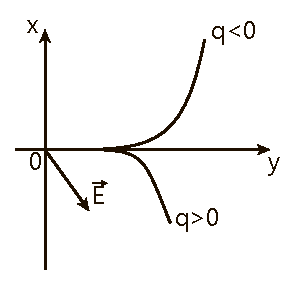
\includegraphics[width=.3\textwidth]{06_electric} \hspace{1em}
%  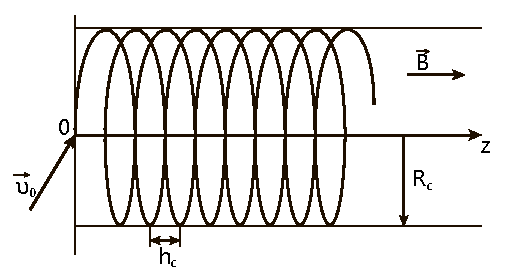
\includegraphics[width=.3\textwidth]{06_magnetic}
  \parbox{.3\textwidth}{\caption{Траектории движения в электрическом поле}
    \label{pic06el}} \hspace{1em}
  \parbox{.3\textwidth}{\caption{Траектории движения в магнитном поле}
    \label{pic06mag}}
\end{figure}

\subquestion{Движение одиночного заряда в однородном статическом электрическом
  поле}

Электрическое поле отсутствует (\( \vec{E} = 0 \)). Выберем ось \( z \) вдоль
вектора магнитной индукции\\ \( \vec{B} = \big\{ 0, 0, B \big\} \). Тогда
\[
  m\vec{a} = q
  \begin{vmatrix}
    \vec{e}_x & \vec{e}_y & \vec{e}_z \\
      \dot{x} &   \dot{y} &   \dot{z} \\
            0 &         0 &         B
  \end{vmatrix}
  = qB\left( \dot{y}\vec{e}_x - \dot{x}\vec{e}_y \right).
\]

В проекции на координатные оси получим
\[
  \left\{
    \begin{array}{l}
      \ddot{x} = \dfrac{q}{m}B\dot{y} = \omega_c\dot{y}, \\[.5em]
      \ddot{y} = -\dfrac{q}{m}B\dot{x} = -\omega_c\dot{x}, \\[.5em]
      \ddot{z} = 0,
    \end{array}
  \right.
\]
где \( \omega_c = qB / m \)~-- циклотронная частота.

Выберем начало координат так, чтобы \( x_0 = y_0 = z_0 = 0 \). Тогда
\( z = v_{0z}t \). Домножим второе уравнение на мнимую единицу \( i \) и сложим
с первым:
\[
  \ddot{x} + i\ddot{y} = \omega_c (\dot{y} - i\dot{x}) =
    -i\omega_c(\dot{x} + i\dot{y}).
\]

Обозначая \( x + iy = u \) получим дифференциальное уравнение:
\[
  \ddot{u} = -i\omega_c\dot{u}.
\]

Его общее решение: \( u = R_0 e^{-i\omega_c t} + C \). Так как \( u(0) = 0 \)
и \( \dot{u}(0) = v_{x0} + iv_{y0} \), то
\[
  u = x + iy = \frac{v_{y0} - iv_{x0}}{\omega_c}
    \Big( 1 - e^{-i\omega_c t} \Big).
\]

Воспользовавшись формулой Эйлера \( e^{-i\alpha} = \cos\alpha - i\sin\alpha \),
получим выражения для \( x \) и \( y \):
\[
  x = \frac{v_{y0}}{\omega_c} \Big( 1 - \cos\omega_c t \Big) +
    \frac{v_{x0}}{\omega_c}\sin\omega_c t, \qquad
  y = -\frac{v_{x0}}{\omega_c} \Big( 1 - \cos\omega_c t \Big) +
    \frac{v_{y0}}{\omega_c}\sin\omega_c t.
\]

Возводя оба равенства в квадрат и складывая, получим:
\[
  \left( x - \frac{v_{y0}}{\omega_c} \right)^2 +
    \left( y + \frac{v_{x0}}{\omega_c} \right)^2 =
    \frac{v_{x0}^2 + v_{y0}^2}{\omega_c^2}.
\]

Это уравнение окружности с центром в точке
\(
  \left(
    \dfrac{v_{y0}}{\omega_c}, -\dfrac{v_{x0}}{\omega_c}
  \right)
\)
и радиусом \( \sqrt{\dfrac{v_{x0}^2 + v_{y0}^2}{\omega_c^2}} \).

Таким образом, траектория заряженной частицы в магнитном поле есть винтовая
линия с шагом \( h_c = v_{z0}T_c = 2\pi v_{z0} / \omega_c \) (рис.~\pic{06mag}).
